\documentclass[../PolyS1.tex]{subfiles}
\begin{document}

La trigonométrie a commencé il y a plus de 2000 ans, lorsque les astronomes ont travaillé sur la mesure des angles et des côtés des triangles.
Le mot \og trigonométrie\fg\ est composé de deux mots grecs \og trigonon\fg\  et \og metron\fg\  qui signifient respectivement triangle et mesure.

La trigonométrie présente un intérêt aussi bien théorique que pratique, car elle est utilisée en mathématiques, en topographie, en ingénierie, en physique, en navigation par satellite, ...

\section{Trigonométrie du triangle}


Soit $ABC$ un triangle rectangle en $C$.

\vspace{1em}
Les rapports $\dfrac{AC}{AB}, \dfrac{BC}{AB},\dfrac{BC}{AC}$ ne dépendent que de l'angle $\widehat{BAC}$ noté $\alpha$ :
\begin{multicols}{2}
\begin{minipage}{0.9\linewidth}
\vspace{2em}
\begin{center}
$\cos\alpha=\dfrac{\text{c\^oté\, adjacent}}{\text{hypoténuse}}=\dfrac{AC}{AB}$
\medskip

$\sin\alpha=\dfrac{\text{c\^oté\, opposé}}{\text{hypoténuse}}=\dfrac{BC}{AB}$
\medskip

$\tan\alpha=\dfrac{\text{c\^oté\, opposé}}{\text{c\^oté\, adjacent}}=\dfrac{BC}{AC}$
\end{center}
\end{minipage}

\begin{tikzpicture}[scale=2, every node/.style={font=\small}]
  % Définition des points
  \coordinate (A) at (0,0);
  \coordinate (C) at (3,0);
  \coordinate (B) at (3,2);

  % Triangle
  \draw[thick] (A) -- (C) -- (B) -- cycle;

  % Angle alpha avec arc propre
  \draw[-, thick] (A) -- ($ (A)!0.8!(C) $);
  \draw[-, thick] (A) -- ($ (A)!0.8!(B) $);
  \pic[draw=black, fill=yellow!40, angle radius=9mm, "$\alpha$"] {angle=C--A--B};

  % Angle beta avec arc propre
  \draw[-, thick] (B) -- ($ (B)!0.8!(C) $);
  \draw[-, thick] (B) -- ($ (B)!0.8!(A) $);
  \pic[draw=black, fill=yellow!40, angle radius=9mm, "$\beta$" ] {angle=A--B--C};

  % Angle droit en C
  \draw (C)+(-0.2,0) -- +(-0.2,0.2) -- +(0,0.2);

  % Longueurs
  \path (A) -- node[below] {$b$} (C);
  \path (C) -- node[right] {$a$} (B);
  \path (A) -- node[above left] {$c$} (B);

  % Points
  \node[below left] at (A) {A};
  \node[below right] at (C) {C};
  \node[above right] at (B) {B};
\end{tikzpicture}

\end{multicols}



 \begin{Prop}\textbf{Propriétés fondamentales}
    \vspace{1em}

\begin{multicols}{2}
\begin{itemize}
\item[] $0<\cos\alpha<1$ et $0<\sin\alpha<1$
\item[] $\cos^2\alpha+\sin^2\alpha=1$
\item[] $\sin(90-\alpha)=\cos\alpha$
\item[] $\dfrac{a}{\sin\alpha}=\dfrac{b}{\sin\beta}$
\end{itemize}
\end{multicols}
\end{Prop}


\newpage

\subsection*{QCM}
\begin{enumerate}
\item $\cos(\alpha)=\dots$
\begin{multicols}{2}
\begin{enumerate}[itemsep=1em]
\item   $\dfrac{\text{c\^oté\, opposé}}{\text{hypoténuse}}$
\item   $\dfrac{\text{c\^oté\, adjacent}}{\text{hypoténuse}}$
\item   $\dfrac{\text{c\^oté\, opposé}}{\text{c\^oté\, adjacent}}$
\item   $\dfrac{\text{c\^oté\, adjacent}}{\text{c\^oté\, opposé}}$
\end{enumerate}
\end{multicols}

\item $\sin(\alpha)=\dots$

\begin{multicols}{2}
\begin{enumerate}[itemsep=1em]
\item   $\dfrac{\text{c\^oté\, opposé}}{\text{hypoténuse}}$
\item   $\dfrac{\text{c\^oté\, adjacent}}{\text{hypoténuse}}$
\item   $\dfrac{\text{c\^oté\, opposé}}{\text{c\^oté\, adjacent}}$
\item   $\dfrac{\text{c\^oté\, adjacent}}{\text{c\^oté\, opposé}}$
\end{enumerate}   
\end{multicols}

\item $\tan(\alpha)=\dots$
\begin{multicols}{2}
\begin{enumerate}[itemsep=1em]
\item   $\dfrac{\text{c\^oté\, opposé}}{\text{hypoténuse}}$
\item   $\dfrac{\text{c\^oté\, adjacent}}{\text{hypoténuse}}$
\item   $\dfrac{\text{c\^oté\, opposé}}{\text{c\^oté\, adjacent}}$
\item   $\dfrac{\text{c\^oté\, adjacent}}{\text{c\^oté\, opposé}}$
\end{enumerate}   
\end{multicols}

\item $\text{cotan}(\alpha)=1/\tan(\alpha) = \dots$

\begin{multicols}{2}
\begin{enumerate}[itemsep=1em]
\item   $\dfrac{\text{c\^oté\, opposé}}{\text{hypoténuse}}$
\item   $\dfrac{\text{c\^oté\, adjacent}}{\text{hypoténuse}}$
\item   $\dfrac{\text{c\^oté\, opposé}}{\text{c\^oté\, adjacent}}$
\item   $\dfrac{\text{c\^oté\, adjacent}}{\text{c\^oté\, opposé}}$
\end{enumerate}     
\end{multicols}
\end{enumerate}  


\section{Le cercle trigonométrique}

\begin{Def}\textbf{Cercle trigonométrique}
    \vspace{1em}

On appelle \emph{cercle trigonométrique} tout cercle dont le rayon est égal à l'unité de longueur et sur lequel on a choisi un sens de rotation \emph{direct} ou sens positif.

On choisit généralement le sens inverse des aiguilles d'une montre.
\end{Def}

\begin{center}


\begin{tikzpicture}[scale=3]
  % Axes
  \draw[->] (-1.2,0) -- (1.4,0);
  \draw[->] (0,-1.2) -- (0,1.4);

  % Cercle trigonométrique
  \draw (0,0) circle(1);

  % Points I, J et O
  \fill (1,0) circle(0.015) node[below right] {$I\,(1\,;\,0)$};
  \fill (0,1) circle(0.015) node[above left] {$J\,(0\,;\,1)$};
  \node at (0.1,-0.1) {$O$};

  % Flèche du sens trigonométrique (au-dessus)
  \draw[->, thick] (0.8,0.8) arc[start angle=45, end angle=75, radius=1.2];
  \node at (0.7,1.1) {\textbf{+}};
\end{tikzpicture}


\end{center}



\subsection{Se repérer sur le cercle trigonométrique}



Dans un repère orthonormal $(O;\overrightarrow{OI};\overrightarrow{OJ})$, on considère le cercle trigonométrique de centre O et la droite $\mathcal{D}$ tangente en $I$ au cercle. Cette droite est {\bf graduée} et {\bf le zéro coïncide avec le point $I$}.




\begin{minipage}{1\linewidth}
\begin{center}
\includegraphics[scale=0.5]{images/enroulement.png}
\end{center}
\end{minipage}


 \begin{Prop}\textbf{Cercle trigonométrique}
    \vspace{1em}

Tout point du cercle trigonométrique est {\bf l'image} d'une {\bf infinité} de réels de la droite $\mathcal{D}$.
\end{Prop}

\begin{bclogo}[couleur = yellow!10, arrondi = 0.1, ombre = true, couleurOmbre=black!30, logo=\bcfeuvert]{Rappel et méthode}

\begin{itemize}
\item   Le périmètre d'un cercle de rayon 1 (un tour complet) vaut $2\pi$.

\item Pour tester si deux réels $x$ et $x'$ ont le même point image sur le cercle trigonométrique, on peut chercher si $x-x'$ est un multiple de $2\pi$ :\newline 
on cherche $k\in\Z$ tel que $x-x'=k.2\pi$.

\end{itemize}
\end{bclogo}



\subsection{Le Radian}

\begin{Def}\textbf{Radian}
    \vspace{1em}

Le \emph{radian} est une unité de mesure des angles. 

La mesure d'un angle correspond à la longueur de l'arc intercepté par l'angle au centre d'un cercle de rayon $1$.


Sur le dessin suivant, l'angle $\widehat{MOM'}$ mesure $\alpha$ radians.

La longueur de l'arc $\overset{\displaystyle\frown}{MM'}$ vaut $\alpha$.
\end{Def}

\begin{center}
% \includegraphics[scale=0.4]{images/radian.png}

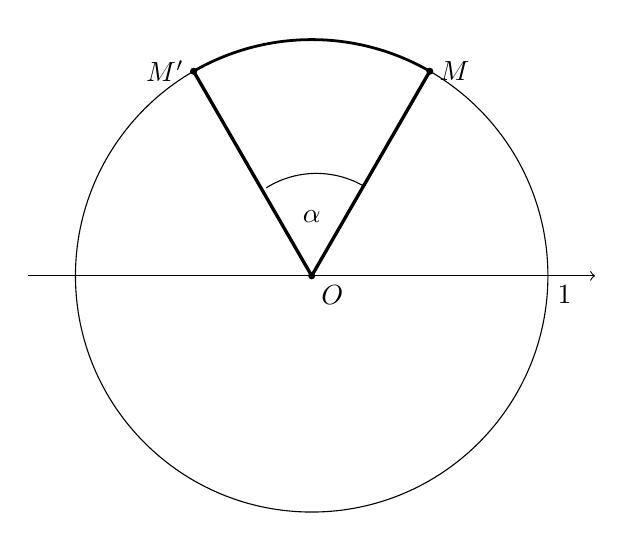
\begin{tikzpicture}[scale=3]
  % Cercle trigonométrique
  \draw (0,0) circle(1);

  % Points du cercle
  \coordinate (O) at (0,0);
  \coordinate (I) at (1,0);
  \coordinate (M) at (60:1);     % angle alpha
  \coordinate (Mp) at (120:1);   % symétrique de M

  % Axes
  \draw[->] (-1.2,0) -- (1.2,0);
  \node[below right] at (I) {$1$};

  % Points
  \fill (O) circle(0.015) node[below right] {$O$};
  \fill (M) circle(0.015) node[right] {$M$};
  \fill (Mp) circle(0.015) node[left] {$M'$};

  % Segments OM et OM' en gras
  \draw[line width=1.2pt] (O) -- (M);
  \draw[line width=1.2pt] (O) -- (Mp);

  % Arc en gras entre M' et M
  \draw[line width=1pt] (Mp) arc[start angle=120, end angle=60, radius=1];

  % Angle alpha
  \draw (0.22,0.38) arc[start angle=60, end angle=122, radius=0.4];
  \node at (0.,0.25) {$\alpha$};
\end{tikzpicture}

\end{center}


La longueur d'un arc de cercle de rayon $R$ et de mesure $\alpha>0$ {\bf exprimé en radians} est égale au produit $\alpha R$ {\bf exprimé dans l'unité de $R$}.


\begin{Prop}\textbf{Mesure d'un angle en radian}
    \vspace{1em}

La mesure d'un angle en radian est \emph{proportionnelle} à la mesure du même angle en degrés.

\noindent Un angle plat mesure $180$ en degrés ou $\pi$ en radians.
\end{Prop}

\newpage

\subsection{Cosinus et sinus d'un nombre réel}

\begin{Def}\textbf{Cosinus et sinus}
    \vspace{1em}

Soit un cercle trigonométrique dans un repère orthonormal $(O;\overrightarrow{OI};\overrightarrow{OJ})$. On considère un nombre réel $x$.


\begin{itemize}
\item[$\bullet$] On appelle \emph{cosinus} de $x$, noté $\cos x$, l'abscisse du point $M$ associée à $x$.
\item[$\bullet$] On appelle \emph{sinus} de $x$ noté $\sin x$, l'ordonnée du point $M$ associée à $x$.
\end{itemize}
\end{Def}


\begin{center}
% \includegraphics[scale=0.4]{images/fonctionTrigo.png}

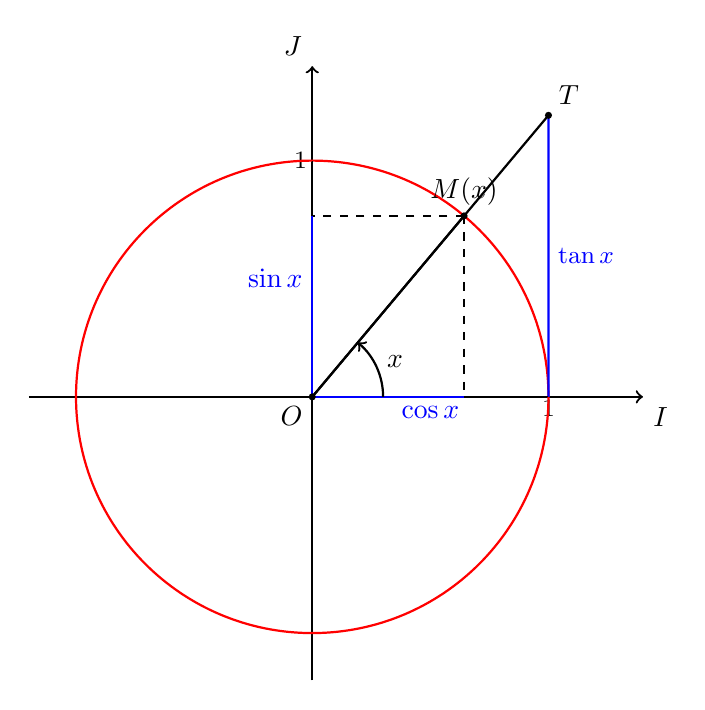
\begin{tikzpicture}[scale=3]
  % Repère
  \draw[->, thick] (-1.2, 0) -- (1.4, 0) node[below right] {$I$};
  \draw[->, thick] (0, -1.2) -- (0, 1.4) node[above left] {$J$};

  % Unités sur les axes
  \node at (1, -0.05) {\small $1$};
  \node at (-0.05, 1) {\small $1$};

  % Cercle trigonométrique
  \draw[red, thick] (0,0) circle(1);

  % Points
  \coordinate (O) at (0,0);
  \coordinate (I) at (1,0);
  \coordinate (J) at (0,1);
  \coordinate (M) at ({cos(50)}, {sin(50)}); % Angle x = 50°
  \coordinate (T) at (1,{tan(50)});
  \coordinate (Mx) at ({cos(50)}, 0);
  \coordinate (Jx) at (0,{sin(50)});

  % Vecteur OM
  \draw[thick] (O) -- (M) node[above] {$M(x)$};
  \fill (M) circle(0.015);

  % Cosinus
  \draw[dashed, thick] (M) -- (Mx);
  \draw[blue, thick] (O) -- (Mx);
  \node[blue, below] at (0.5, 0) {$\cos x$};

  % Sinus
  \draw[dashed, thick] (M) -- (Jx);
  \draw[blue, thick] (O) -- (Jx);
  \node[blue, left] at (0, 0.5) {$\sin x$};

  % Tangente
  \draw[thick] (O) -- (T) node[above right] {$T$};
  \draw[blue, thick] (1,0) -- (T);
  \fill (T) circle(0.015);
  \node[blue, right] at (1, {0.5*tan(50)}) {\small $\tan x$};

  % Pointillés
  \draw[dashed] (Mx) -- (1,0);
  \draw[dashed] (Jx) -- (0,1);

  % Angle x (arc fléché)
  \draw[->, thick] (0.3,0) arc[start angle=0, end angle=50, radius=0.3];
  \node at (0.35, 0.15) {$x$};

  % Origine et points importants
  \fill (O) circle(0.015) node[below left] {$O$};
  % \fill (I) circle(0.015);
  % \fill (J) circle(0.015);

\end{tikzpicture}

\end{center}

\subsection{Propriétés}

\begin{Ex}Valeurs remarquables:
\begin{center}
\begin{tabular}{|c|c|c|c|}
\hline
degrés & radians & sinus & cosinus\\
\hline
&&&\\
$0$ & $0$ & $0$ & $1$ \\
&&&\\
\hline
&&&\\
 & ${\pi}/{6}$ & ${1}/{2}$ &  \\
&&&\\
\hline
&&&\\
$45$ &  &  & ${\sqrt{2}}/{2}$ \\
&&&\\
\hline
&&&\\
& ${\pi}/{3}$ & $\sqrt{3}/{2}$ & \\
&&&\\
\hline
&&&\\
$90$ &  & & $0$ \\
&&&\\
\hline
&&&\\
& $\pi$ & $0$ & $-1$ \\
&&&\\
\hline
\end{tabular}
\end{center}

\end{Ex}

\begin{Ex} 

Figure à compléter:

\begin{center}
\includegraphics[scale=0.4]{images/completer.png}
\end{center}
\end{Ex}


 \begin{Prop}\textbf{Propriétés}
    \vspace{1em}

Pour tout nombre réel $x$,
\begin{multicols}{2}
\begin{itemize}
\item[] $\cos^2{x}+\sin^2{x}=1$
\item[] $-1 \leq \cos{x} \leq 1$\newline $-1 \leq \sin{x} \leq 1$
\item[] $\cos{(-x)}=\cos{(x)}$
\item[] $\sin{(-x)}=-\sin{(x)}$
\end{itemize}
\end{multicols}
\end{Prop}

\begin{Ex}Placer les angles $x+\pi,\ \pi-x,\ x+\frac{\pi}{2},\  \frac{\pi}{2}-x$\\
\begin{center}
\includegraphics[scale=0.4]{images/completer2.png}
\end{center}
\end{Ex}


\begin{Ex}

Pour tout nombre réel $x$ :

\begin{itemize}
\item[$\bullet$] $\cos{(x+\pi)}=\hspace{4cm}\sin{(x+\pi)}=$
\item[$\bullet$] $\cos{(\pi-x)}=\hspace{4cm}\sin{(\pi-x)}=$
\item[$\bullet$] $\cos{\left(x+\frac{\pi}{2}\right)}=\hspace{4cm}\sin{\left(x+\frac{\pi}{2}\right)}=$
\item[$\bullet$] $\cos{\left(\frac{\pi}{2}-x\right)}=\hspace{4cm}\sin{\left(\frac{\pi}{2}-x\right)}=$
\end{itemize}
\end{Ex}


\subsection{QCM}
\begin{enumerate}[itemsep=2em]
\item Le cercle trigonométrique a ...

\begin{enumerate}
\item   pour centre l'origine et pour rayon $1$.
\item   pour centre l'origine et pour diamètre $1$.
\item   pour centre l'origine et pour rayon $2\pi$.
\item   pour centre l'origine et pour diamètre $2\pi$.
\end{enumerate}

\newpage


\item Sur le cercle trigonométique, un point $M$ associé à l'angle $x$ a $\dots$ 
\begin{enumerate}
\item   pour abscisse $\cos(x)$ et ordonnée $\sin(x)$.
\item   pour abscisse $\sin(x)$ et ordonnée $\cos(x)$.
\item   pour abscisse $\tan(x)$ et ordonnée $\sin(x)$.
\item   pour abscisse $\cos(x)$ et ordonnée $\tan(x)$.
\end{enumerate}   

\item $\sin\left(\dfrac{\pi}{4}\right)=\cdots$
\begin{multicols}{3}
\begin{enumerate}
\item   $\dfrac{\sqrt{2}}{2}$
\item  $\dfrac{1}{2}$
\item    $\dfrac{\sqrt{3}}{2}$
\item   $1$
\item $0$
\end{enumerate}   
\end{multicols}

\item $\sin\left(\dfrac{18\pi}{4}\right)=\cdots$
\begin{multicols}{3}
\begin{enumerate}
\item   $\dfrac{\sqrt{2}}{2}$
\item  $\dfrac{1}{2}$
\item   $\dfrac{\sqrt{3}}{2}$
\item   $1$
\item $0$
\end{enumerate}  
\end{multicols}


\item  La mesure principale de $\dfrac{28\pi}{3}$ est
\begin{multicols}{2}
\begin{enumerate}
\item   $\dfrac{2\pi}{3}$
\item  $-\dfrac{2\pi}{3}$
\item   $\dfrac{\pi}{3}$
\item   $-\dfrac{\pi}{3}$

\end{enumerate}  
\end{multicols}

\item  Soit $x$ un réel quelconque, $\cos(x+2\pi)=\cdots$
\begin{multicols}{2}
\begin{enumerate}
\item   $\cos(x)$
\item  $-\cos(x)$
\item   $\sin(x)$
\item   $-\sin(x)$

\end{enumerate}
\end{multicols}


\item  Soit $x$ un réel quelconque, $\cos(x+\pi)=\cdots$
\begin{multicols}{2}
\begin{enumerate}
\item   $\cos(x)$
\item  $-\cos(x)$
\item   $\sin(x)$
\item   $-\sin(x)$

\end{enumerate}
\end{multicols}

\item  Soit $x$ un réel quelconque, $\sin(-x)=\cdots$
\begin{multicols}{2}
\begin{enumerate}
\item   $\cos(x)$
\item  $-\cos(x)$
\item   $\sin(x)$
\item   $-\sin(x)$

\end{enumerate}
    \end{multicols}

\end{enumerate}  

\newpage


\section{Fonctions circulaires}
\subsection{Fonction cosinus}
\begin{Def} \textbf{La fonction cosinus}
    \vspace{1em}

On définit une fonction de $\R$ dans l'intervalle $[-1; 1]$ qui à tout nombre réel $x$ associe le cosinus du nombre $x$:
$$\cos: \begin{array}{ccl}
\R&\to&[-1;1]\\
x&\mapsto&\cos x
\end{array}$$
\end{Def}


 \begin{Prop}\textbf{Propriétés}
    \vspace{1em}

La fonction cosinus 
\begin{itemize}

\item est continue sur $\mathbb{R}$
\item est périodique de période $2\pi :$
$\quad \forall k\in\Z,\ \cos (x+2k\pi)=\cos x$
\item est paire : $\forall x\in\R \quad \cos (-x)=\cos x$
\item est indéfiniment dérivable :
$$\forall x\in\R,\ (\cos x)'=-\sin x, \qquad 
 \forall n\in\N^*,\ (\cos x)^{(n)}=\cos\left(x+n\dfrac{\pi}{2}\right)$$
\end{itemize}

\end{Prop}

\begin{center}

\begin{tabular}{|c|lcccr|}
\hline
&&&&&\\
$x$ & $0$ & & $\frac{\pi}{2}$ & & $\pi$ \\
&&&&&\\
\hline
 & $1$ & & & & \\
$\cos{x}$ & & {\unitlength=1cm
     \begin{picture}(1.1,1.2)(0,0)
     \put(0,1.2){\vector(1,-1){1}}
     \end{picture}} & $0$ & & \\
 & & & & 
      {\unitlength=1cm
     \begin{picture}(1.1,1.2)(0,0)
     \put(0,1.2){\vector(1,-1){1}}
     \end{picture}}&  $-1$ \\
\hline
\end{tabular}
    
\end{center}

\begin{center}
\includegraphics[scale=0.5]{images/cosinus.png}
\end{center}


 
\exo[1]{Questions}
\begin{enumerate}
\item la fonction cosinus est-elle monotone ?
\item les fonctions $x\longmapsto x\cos x$ et $x\longmapsto \dfrac{\cos x}{x}$ admettent une limite en en 0 ? En $+\infty$ ?
\end{enumerate}


\subsection{Limites à connaître}
$$ \lim_{x\ \to\ 0}\dfrac{1-\cos x}{x^2/2}=1, \qquad \lim_{x\ \to\ 0}\dfrac{1-\cos x}{x}=0.$$

\subsection{Fonction sinus}

\begin{Def}\textbf{La fonction sinus}
    \vspace{1em}

On définit une fonction de $\R$ dans l'intervalle $[-1; 1]$ qui à tout nombre réel $x$ associe le sinus du nombre $x$:
$$
\sin : \begin{array}{ccl}
\R&\to&[-1;1]\\
x&\mapsto&\sin x
\end{array}$$
\end{Def}


 \begin{Prop}\textbf{Propriétés}
    \vspace{1em}

La fonction sinus
\begin{itemize}
\item est continue sur $\mathbb{R}$
\item est périodique de période $2\pi :$
$\quad \forall k\in\Z,\ \sin (x+2k\pi)=\sin x$
\item est impaire : $\forall x\in\R \quad \sin (-x)=-\sin x$
\item est indéfiniment dérivable :
$$\forall x\in\R,\ (\sin x)'=\cos x, \qquad 
 \forall n\in\N^*,\ (\sin x)^{(n)}=\sin\left(x+n\dfrac{\pi}{2}\right)$$
\end{itemize}

\end{Prop}

\begin{tabular}{|c|lcccr|}
\hline
&&&&&\\
$x$ & $0$ & & $\frac{\pi}{2}$ & & $\pi$ \\
&&&&&\\
\hline
 & & &  & & \\
 $\sin{x}$ &&&$1$&&\\
& $0$ & {\unitlength=1cm
     \begin{picture}(1.1,1.2)(0,0)
     \put(0.1,0.2){\vector(1,1){1}}
     \end{picture}} & & {\unitlength=1cm
     \begin{picture}(1.1,1.2)(0,0)
     \put(0,1.2){\vector(1,-1){1}}
     \end{picture}} & $0$ \\
\hline
\end{tabular}

\begin{minipage}{1\linewidth}
\begin{center}
\includegraphics[scale=0.5]{images/sinus.png}
\end{center}
\end{minipage}


\newpage


\exo[1]{Questions} 

\begin{enumerate}
\item la fonction sinus est-elle monotone ?
\item les fonctions $x\longmapsto x\sin x$ et $x\longmapsto \dfrac{\sin x}{x}$ admettent une limite en 0 ? En $+\infty$ ?
\end{enumerate}

\subsection{Limites à connaître}
$$\lim_{x\ \to\ 0}\dfrac{\sin x}{x}=1$$

%% TAN
\subsection{Fonction tangente}
\begin{Def}\textbf{La fonction tangente}
    \vspace{1em}    

On note $D_f$ l'ensemble 
$$D_f=\left\{x\in\mathbb{R}\text{ tels que }\ x\neq\dfrac{\pi}{2}+k\pi,\ k\in\mathbb{Z}\right\}\,.$$
On définit une fonction de $D_f$ dans l'intervalle $[-1, 1]$ qui à tout nombre réel $x$ associe la tangente du nombre $x$:
$$
\tan:\begin{array}{rcl}
D_f&\to&\mathbb{R}\\
x&\longmapsto&\tan x=\dfrac{\sin x}{\cos x}
\end{array}$$
\end{Def}


\begin{Prop}\textbf{Propriétés}
    \vspace{1em}

La fonction tangente 
\begin{itemize}
\item est continue sur tout intervalle de $D_f$
\item est périodique de période $\pi$ : $\quad\forall k\in\Z \quad \tan (x+k\pi)=\tan x$
\item est impaire : $\tan (-x)=-\tan x$
\item est dérivable :
$$\forall x\in D_f,\ (\tan x)'=1+\tan^2 x=\dfrac{1}{\cos^2 x}$$
\end{itemize}

\end{Prop}

\begin{center}
 
\begin{tabular}{|c|lcccc|}
\hline
%&&&&&\\
$x$ & $-\frac{\pi}{2}$ & & 0 & & $\frac{\pi}{2}$\\
%&&&&&\\
\hline
 & & &  & &$+\infty$ \\
 & & &  & $\nearrow$ & \\
$\tan{x}$ & & & 0  & & \\
&&$\nearrow$ &&&\\
& $-\infty$ & & & & \\
\hline
\end{tabular}
   
\end{center}

\begin{center}
\includegraphics[scale=0.5]{images/tangente.png}
\end{center}

\subsection{QCM}

\begin{enumerate}[label=\textbf{Q\arabic*.}]

\item La fonction \( \cos \) est :
\begin{multicols}{2}
\begin{itemize}
    \item[1.] Continue et dérivable sur \( \mathbb{R} \)
    \item[2.] Strictement croissante sur \( [0, \pi] \)
    \item[3.] Bornée par 1 et -1
    \item[4.] Périodique de période \( \pi \)
\end{itemize}
\end{multicols}

\item La fonction \( \sin \) est :
\begin{multicols}{2}
\begin{itemize}
    \item[1.] Strictement croissante sur \( [0, \frac{\pi}{2}] \)
    \item[2.] Impaire
    \item[3.] De période \( 2\pi \)
    \item[4.] Convexe sur \( [0, \frac{\pi}{2}] \)
\end{itemize}
\end{multicols}

\item La fonction tangente \( \tan \) est définie sur :
\begin{multicols}{2}
\begin{itemize}
    \item[1.] \( \mathbb{R} \)
    \item[2.] \( \mathbb{R} \setminus \left\{ \frac{\pi}{2} + k\pi \; | \; k \in \mathbb{Z} \right\} \)
    \item[3.] \( ] -\frac{\pi}{2}, \frac{\pi}{2} [ \)
    \item[4.] Aucun intervalle de longueur \( \pi \)
\end{itemize}
\end{multicols}

\item On a les limites suivantes :
\begin{multicols}{2}
\begin{itemize}
    \item[1.] \(\displaystyle \lim_{x \to 0} \frac{\sin(x)}{x} = 1 \)
    \item[2.] \(\displaystyle \lim_{x \to 0} \frac{1 - \cos(x)}{x} = 0 \)
    \item[3.] \(\displaystyle \lim_{x \to \frac{\pi}{2}^-} \tan(x) = +\infty \)
    \item[4.] \(\displaystyle \lim_{x \to +\infty} \cos(x) \) existe
\end{itemize}
\end{multicols}

\item Les dérivées des fonctions trigonométriques usuelles sont :
\begin{multicols}{2}
\begin{itemize}
    \item[1.] \( (\cos(x))' = -\sin(x) \)
    \item[2.] \( (\sin(x))' = \cos(x) \)
    \item[3.] \( (\tan(x))' = 1 + \tan^2(x) \)
    \item[4.] \( (\tan(x))' = \frac{1}{\cos^2(x)} \)
\end{itemize}
\end{multicols}

\item Concernant la croissance des fonctions :
\begin{multicols}{2}
\begin{itemize}
    \item[1.] \( \sin \) est croissante sur \( [-\frac{\pi}{2}, \frac{\pi}{2}] \)
    \item[2.] \( \cos \) est décroissante sur \( [0, \pi] \)
    \item[3.] \( \tan \) est strictement croissante sur chacun de ses intervalles de définition
    \item[4.] \( \cos \) est croissante sur \( [\pi, 2\pi] \)
\end{itemize}
\end{multicols}

\newpage


\item À propos du caractère borné :
\begin{multicols}{2}
\begin{itemize}
    \item[1.] \( \cos(x) \) est bornée sur \( \mathbb{R} \)
    \item[2.] \( \sin(x) \) est bornée par \( [-1,1] \)
    \item[3.] \( \tan(x) \) est bornée sur \( \mathbb{R} \)
    \item[4.] \( \tan(x) \) est non bornée sur chaque intervalle de définition
\end{itemize}
\end{multicols}

\item À propos des parités :
\begin{multicols}{2}
\begin{itemize}
    \item[1.] \( \cos \) est paire
    \item[2.] \( \sin \) est impaire
    \item[3.] \( \tan \) est paire
    \item[4.] \( \tan \) est impaire
\end{itemize}
\end{multicols}

\end{enumerate}


\subsection{Exercices}

\vspace{1em}
\hrule
\vspace{1em}

\exo[3]{Produit scalaire}
 On considère dans un repère orthonormé les vecteurs $\overrightarrow u $ et $\overrightarrow v $ du schéma ci-dessous. 
 
 \begin{enumerate}
\item En utilisant les deux expressions du produit scalaire appliqué à $\overrightarrow u $ et $\overrightarrow v $, démontrer que $$\cos (a-b)=\cos a\cos b+\sin a\sin b\,. $$

\begin{center}
\includegraphics[scale=0.5]{images/cercle-trigonometrique-addition-cosinus}
\end{center}

\item Démontrer que $\tan(a+b)=\dfrac{\tan a+\tan b}{1-\tan a\tan b}$. En déduire $\tan 2a$.
\item Exprimer $\tan\left(\dfrac{\pi}{4}+a\right)-\tan\left(\dfrac{\pi}{4}-a\right)$ en fonction de $\tan2a$.
\item Montrer que 
$$1+\sin4x-\cos4x=2\sqrt2\sin(2x)\sin\left(\dfrac{\pi}{4}+2x\right).$$
\item \begin{enumerate}
\item Vérifier la formule $\cot x-2\cot 2x=\tan x$.
\item En déduire que 
\begin{align*}
S_n&=\tan (x)+2\tan(2x)+4\tan(4x)+\dots+2^n\tan(2^nx)\\
&= \cot x-2^{n+1}\cot2^{n+1}x.
\end{align*}
\end{enumerate}
\item Soit $x\in[0;\frac{\pi}{2}[$ tel que $\cos x=\dfrac{\sqrt 2+\sqrt 6}{4}$.\begin{enumerate}
\item Calculer $\cos 2x$.
\item En déduire la valeur de $x$.
\end{enumerate}
\end{enumerate}


\vspace{1em}
\hrule
\vspace{1em}


\section{\'Equations trigonométriques}

\subsection{\'Equations du type $\cos x=a$ et $\sin x=b$}
{\bf Si $a$, $b$ sont des valeurs remarquables,} on peut obtenir une expression exacte de la solution.

Résoudre dans $\mathbb{R}$ les équations suivantes :$$\cos x=\dfrac{1}{2},\qquad\sin x=\dfrac{\sqrt 2}{2},\qquad\cos x=-\dfrac{\sqrt 2}{2},\qquad\sin x=-\dfrac{1}{2}.$$

{\bf Sinon,} on utilise la calculatrice et les fonctions réciproques $\cos^{-1}$ et $\sin^{-1}$ ainsi que les propriétés des fonctions cosinus et sinus.

\subsection{\'Equations du type $\cos x=\cos y$, $\sin x=\sin y$, $\tan x=\tan y$}

\begin{bclogo}[couleur = yellow!10, arrondi = 0.1, ombre = true, couleurOmbre=black!30, logo=\bcfeuvert]{Résultats à connaître}
$$\boldsymbol{\cos(x)=\cos(y) \Longleftrightarrow x=\pm y + 2k\pi\quad(k\in\Z)}$$

$$\boldsymbol{\sin(x)=\sin(y) \Longleftrightarrow x=y + 2k\pi\textrm{ ou } x=\pi-y+ 2k\pi \quad(k\in\Z)}$$

$$\boldsymbol{\tan(x)=\tan(y) \Longleftrightarrow x=y + k\pi\quad(k\in\Z)}$$
\end{bclogo}

\paragraph{Autres types d'équations se ramenant aux précédentes :}

\begin{enumerate}
\item $\sin u=\cos v\Longleftrightarrow \sin u=\sin \left(\dfrac{\pi}{2}-v\right).$
\item $\sin u=-\sin v\Longleftrightarrow \sin u=\sin (-v).$
\item $\sin u=-\cos v\Longleftrightarrow \sin u=\sin \left(v-\dfrac{\pi}{2}\right).$
\end{enumerate}
%\newpage

\exo[2]{\'Equations}
Résoudre dans $\mathbb{R}$ les équations suivantes :

$$\cos x=\cos\left(\frac{\pi}{2}-x\right), \qquad\sin 3x=\sin x, \qquad\tan^2x =1$$





\subsection{\'Equations du type $f(\cos x,\sin x,\tan x)=0$}
On peut distinguer deux familles de méthodes :
\begin{itemize}
\item celles qui ramènent l'équation initiale à une équation simple dans laquelle n'intervient plus qu'une seule fonction circulaire. Il faut utiliser les formules {\bf d'addition, de duplication, de linéarisation}.
\item celles qui introduisent un changement de variable, comme $t=\tan\dfrac{x}{2}$, avant de ramener à une équation simple dans laquelle n'intervient plus qu'une seule fonction circulaire ou la variable $t$.\end{itemize}



\paragraph{Résoudre $a\cos x+b\sin x=c$.}\hfil\break
\begin{small}

\begin{Ex}
\textbf{ $\cos x-\sin x=\sqrt{\dfrac{3}{2}}$.}\\
\begin{enumerate}
\item L'équation est équivalente à
$$\sqrt{2}\left(\dfrac{1}{\sqrt{2}}\cos x-\dfrac{1}{\sqrt{2}}\sin x\right)=\sqrt{\dfrac{3}{2}}$$
qui équivaut aussi à
$$\dfrac{1}{\sqrt{2}}\cos x-\dfrac{1}{\sqrt{2}}\sin x=\dfrac{\sqrt 3}{2}.$$

\item On définit $\phi$ par : $\cos\phi=\dfrac{1}{\sqrt 2}$ et $\sin\phi=-\dfrac{1}{\sqrt 2}$. Donc $\phi=-\dfrac{\pi}{4}$.
\item L'équation est équivalente à 
$$\cos\left(-\frac{\pi}{4}\right)\cos x+\sin\left(-\frac{\pi}{4}\right)\sin x=\dfrac{\sqrt 3}{2},$$
\item c'est-à-dire\\
$\cos\big(x-(-\pi/4)\big)=\dfrac{\sqrt 3}{2}$, soit $$\cos(x+\pi/4)=\dfrac{\sqrt 3}{2}.$$ 

Et $\dfrac{\sqrt 3}{2}=\cos(\pi/6)$.
\item Alors\\
$$x+\pi/4=\pi/6\ [2\pi] \quad \text{ ou }\quad x+\pi/4=-\pi/6\ [2\pi]$$
C'est-à-dire
$$x=-\pi/4+\pi/6\ [2\pi] \quad \text{ ou }\quad x=-\pi/4-\pi/6\ [2\pi]$$

Finalement :
$$x=-\pi/12\ [2\pi] \quad \text{ ou }\quad x=-5\pi/12\ [2\pi].$$
\end{enumerate}
\end{Ex}

\end{small}


\begin{bclogo}[couleur = yellow!10, arrondi = 0.1, ombre = true, couleurOmbre=black!30, logo=\bcfeuvert]{En résumé }
\begin{itemize}
\item L'équation est équivalente à
$$\dfrac{a}{\sqrt{a^2+b^2}}\cos x+\dfrac{b}{\sqrt{a^2+b^2}}\sin x=\dfrac{c}{\sqrt{a^2+b^2}}.$$
\item On définit $\phi$ par : $\cos\phi=\dfrac{a}{\sqrt{a^2+b^2}}$ et $\sin\phi=\dfrac{b}{\sqrt{a^2+b^2}}$.
\item L'équation est équivalente à $\cos(x-\phi)=\dfrac{c}{\sqrt{a^2+b^2}}$, qui n'a des solutions que si
$$-1\leq\dfrac{c}{\sqrt{a^2+b^2}}\leq 1.$$
\item On identifie, si possible, $\cos(x-\phi)$ au cosinus d'un angle remarquable, on détermine $x-\phi$ puis $x$.
\end{itemize}
\end{bclogo}





\subsection{Exercices :}


\vspace{1em}
\hrule
\vspace{1em}


\exo[3]{\'Equations variées}

Résoudre les équations suivantes.
\begin{enumerate}
\item $12\cos^2x-8\sin^2x=2$ (ramener l'équation à une seule fonction circulaire...)
%\item $2\sin^3x-17\sin^2x+7\sin x+8=0$ (effectuer le changement de variable $t=\sin x$...)
\item $2\sin^2 x+3\cos x=0$ (poser $t=\cos x$ puis se ramener à un équation du second degré)
\item $\cos 2x+2\sin x\cos x=0$ (penser à introduire $\sin2x$...)
\item $\sqrt 3\cos^2x+2\sin x\cos x-\sqrt 3\sin^2x=\sqrt 2$ (utiliser les formules de l'angle double...)
\item $\cos x+\sin x=-1$ %(noter que $\pi$ est solution, poser alors pour tout $x\neq\pi, t=\tan\dfrac{x}{2}$ et utiliser que $\cos x=\dfrac{1-t^2}{1+t^2}$ et $\sin x =\dfrac{2t}{1+t^2}$).
\item $\cos x+\cos 3x=0$
\end{enumerate}
$\,$


\vspace{1em}
\hrule
\vspace{1em}

\section{\'Etude de fonction}

\begin{Ex}

On étudie la fonction $f$ définie par $x\mapsto f(x)=\cos^2x\sin2x$.

\begin{enumerate}
\item Ensemble de définition : $\R$.
\item \textbf{Périodicité} : 

$$
    f(x+\pi)
    =\cos^2(x+\pi)\sin\big(2(x+\pi)\big)
$$
donc $$
    f(x+\pi) =(-\cos x)^2\sin(2x+2\pi)
    =\cos^2x\sin 2x
    =f(x)
$$

La période est $\pi$. \underline{On restreint l'étude de $f$ à un intervalle d'amplitude $\pi$},\newline  par exemple $\left[-\dfrac{\pi}{2},\dfrac{\pi}{2}\right]$.

\item \textbf{Parité} : $$f(-x)=\cos^2(-x)\sin(2(-x))=\cos^2x\sin(-2x)$$
donc 
$$
f(-x)=\cos^2x(-\sin2x)=-\cos^2x\sin2x=-f(x)$$ 
La fonction $f$ est impaire. \underline{On restreint l'étude de $f$ à l'intervalle} $\left[0,\dfrac{\pi}{2}\right]$. 

On complétera la courbe par une symétrie de centre O.
\item \textbf{Dérivée} : \'Ecrivons $f(x)=2\cos^3x\sin x$. Alors : \begin{eqnarray*}
f'(x)&=&6\cos^2x(-\sin x)\sin x+2\cos^3x\cos x\\
&=&-6\cos^2x\sin ^2x+2\cos^4x\\
&=&2\cos^2x(-3\sin^2x+\cos^2x)\\
&=&2\cos^2x(-3\sin^2x+1-\sin^2x)\\
&=&2\cos^2x(1-4\sin^2x)\\
&=&2\cos^2x(1-2\sin x)(1+2\sin x)
\end{eqnarray*}

La résolution de $f'(x)=0$ sur $\left[0,\dfrac{\pi}{2}\right]$ donne comme solutions $\dfrac{\pi}{6}$ et $\dfrac{\pi}{2}$. 

On déduit le signe de $f'(x)$ sur les intervalles $\left[0,\dfrac{\pi}{6}\right]$ et $\left[\dfrac{\pi}{6},\dfrac{\pi}{2}\right]$.
\item \textbf{Monotonie} :

$$\begin{tabular}{|c|lcccr|}
\hline
$x$ & $0$ & & $\pi/6$ & & $\pi/2$ \\
\hline
$f'(x)$& & + & 0 & - & \\
\hline& & &  &  & \\
$f$ &&&$3\sqrt3/8$&&\\
& $0$ & {\unitlength=1cm
     \begin{picture}(1.1,1.2)(0,0)
     \put(0.1,0.2){\vector(1,1){1}}
     \end{picture}} & & {\unitlength=1cm
     \begin{picture}(1.1,1.2)(0,0)
     \put(0,1.2){\vector(1,-1){1}}
     \end{picture}} & $0$ \\
\hline
\end{tabular}$$

\end{enumerate}

\end{Ex}

\section{Exercices}

\vspace{1em}
\hrule
\vspace{1em}

\exo[2]{\'Etude de fonctions}

\'Etudier les fonction suivantes. $$x\mapsto f(x)=\dfrac{\cos2x}{\cos x},\qquad  x\mapsto g(x)=1-8\cos x-4\cos2x,\qquad x\mapsto h(x)=\dfrac{\sin2x}{\cos^2 (2x)}.$$



\vspace{1em}
\hrule
\vspace{1em}

\exo[2]{Déterminer des coefficients}
\medskip

On considère la fonction $f$ définie sur $\R$ par : $f(x)=(ax+b)e^{cx}$, o\`u $a,b,c$ sont trois nombres réels que l'on va déterminer.

Dans un repère du plan, on sait que la courbe représentative de $f$ contient les points $(1;0)$ et $(0;1/3)$. Par ailleurs, cette courbe admet une tangente parallèle \`a l'axe des abscisses au point d'abscisse $2/3$.

En utilisant les différentes informations de l'énoncé, déterminer la valeur de $a,b,c$.

\vspace{1em}
\hrule
\vspace{1em}

%\exo{
%
%On juxtapose 3 carrés de côté 1 comme sur la figure ci-dessous :
%\begin{center}
%\begin{pspicture}
%%\psframe(0,0)(6,2)
%%\psline(2,0)(2,2)\psline(4,0)(4,2)\psline[linestyle=dashed](0,0)(6,2)\psline[linestyle=dashed](2,0)(6,2)
%%\pswedge[fillstyle=solid,fillcolor=yellow](0,0){1}{0}{18.8}\pswedge[fillstyle=solid,fillcolor=green](2,0){1}{0}{26.2}
%%\uput[r](1,0.2){$\alpha$}\uput[r](3,0.3){$\beta$}
%%\end{pspicture}
%\end{center}
%\begin{enumerate}
%\item Calculer $\cos\alpha$, $\sin\alpha$, $\cos\beta$, $\sin\beta$.
%\item Montrer que $\alpha+\beta$ est un angle remarquable.
%\end{enumerate}
%\vspace{1em}
%\hrule
%\vspace{1em}
%
%}
\exo[2]{Tour}

Une tour est entourée par un large fossé comme le montre le dessin ci-dessous :

\begin{center}
    \includegraphics{images/Tour}
\end{center}

En se situant en A, l'angle $\widehat{MAN}$ vaut $42^{o}$. En reculant de 10 mètres (AB = 10) et en se positionnant en  B l'angle $\widehat{MBN}$ vaut $27^{o}$. Les triangles AMN et BMN sont rectangles en M (aplomb de N).

\begin{enumerate}
\item En exprimant MN de deux fa\c cons différentes (\`a l'aide de tangentes d'angle), calculer la longueur AM.
\item En déduire la hauteur de la tour.
\end{enumerate}
\vspace{1em}
\hrule
\vspace{1em}



\exo[2]{Duplication}

\begin{enumerate}
\item \`A l'aide des formules de duplication, donner les valeurs exactes de $\cos^2\dfrac{5\pi}{8}$ et $\sin^2\dfrac{5\pi}{8}$.
\item Identifier un intervalle dans $[0;2\pi]$ auquel appartient $\dfrac{5\pi}{8}$ qui permette de déterminer le signe de son cosinus et celui de son sinus.
\item En déduire les valeurs exactes de $\cos\dfrac{5\pi}{8}$ et $\sin\dfrac{5\pi}{8}$.
\end{enumerate}

\vspace{1em}
\hrule
\vspace{1em}

\exo[3]{\'Egalités}

\begin{enumerate}
\item Démontrer les égalités suivantes en précisant \`a chaque fois leur domaine de validité :
	\begin{enumerate}
	\item $\cos^4 x-\sin^4 x=\cos(2x)$
	\item $\dfrac{\sin 3x}{\sin x}-\dfrac{\cos 3x}{\cos x}=2$
	\item $\sin\left(x-\frac{2\pi}{3}\right)+\sin x+\sin\left(x+\frac{2\pi}{3}\right)=0$
	\item $\tan\left(\frac{\pi}{4}+x\right)+\tan\left(\frac{\pi}{4}-x\right)=\frac{2}{\cos(2x)}$
	\item $\dfrac{1}{\tan x}-\tan x=\frac{2}{\tan(2x)}$
	\end{enumerate}
\item \begin{enumerate}
	\item Pour tout nombre réel $x\not\in\left\{-\dfrac{\pi}{4}+k\pi, k\in\Z\right\}$ établir la formule : 
    $$\tan^2\left(\dfrac{\pi}{4}-x\right)=\dfrac{1-\sin(2x)}{1+\sin2x}.$$
	\item On considère les nombres réels $a$ et $b$ tels que $$0<a<\dfrac{\pi}{2}\text{ et } 0<b<\dfrac{\pi}{2}\text{ et } \tan a=\dfrac{1}{7}\text{ et } \tan b=2.$$

	Déterminer $c$ tel que $c=a+2b$.
	\end{enumerate}
\end{enumerate}
\vspace{1em}
\hrule
\vspace{1em}

\exo[2]{\'Etude de fonction}

Soit $f$ la fonction définie par $f:x\longmapsto\dfrac{\cos x}{1+\sin x}$.

\begin{enumerate}
\item Déterminer le domaine de définition $D_f$ de $f$.
\item La fonction $f$ est-elle périodique ? paire ? impaire ?
\item Déterminer $f'(x)$. En déduire le sens de variation de $f$ sur $\left]-\dfrac{\pi}{2};\dfrac{\pi}{2}\right[$.
\end{enumerate}
%%%
%%%%
%%%%%
%\newpage
%
%\textbf{\Large{Corrigé}}
%\vspace{1cm}
%
%\underline {\ding{110}\, \bf{Exercice 1}}
%
%De l'information que la courbe représentative de $f$ contient les points $(1;0)$ et $(0;1/3)$, on déduit que $$\left\{\begin{array}{l}(a+b)e^c=0\\b=1/3\end{array}\right.\Longleftrightarrow\left\{\begin{array}{l}a+b=0 \,(car\, e^c\neq0)\\b=1/3\end{array}\right.$$
%
%On en déduit que $a=-1/3$ et $b=1/3$. Et $$f(x)=\frac{1}{3}(-x+1)e^{cx}.$$
%
%Ainsi, $f'(x)=\frac{1}{3}\left(-e^{cx}+(-x+1)ce^{cx}\right)=\frac{1}{3}\left(e^{cx}(-1-(x+1)c\right)$.
%
%Comme $f'(2/3)=0$, on déduit que $-1-(2/3+1)c=0$ (car $e^{c(2/3)}\neq0$). D'oé $c=3$.
%
%Au final, $$f(x)=\frac{1}{3}(-x+1)e^{3x}.$$
%\vspace{1em}
%
%\underline {\ding{110}\, \bf{Exercice 2}}
%
%\begin{enumerate}
%\item $\cos\alpha=\dfrac{3}{\sqrt{3^2+1}}=\dfrac{3}{\sqrt{10}}$, $\sin\alpha=\dfrac{1}{\sqrt{3^2+1}}=\dfrac{1}{\sqrt{10}}$, $\cos\beta=\dfrac{2}{\sqrt{2^2+1}}=\dfrac{2}{\sqrt{5}}$, $\sin\beta=\dfrac{1}{\sqrt{2^2+1}}=\dfrac{1}{\sqrt{5}}$.
%\item $\cos(\alpha+\beta)=\cos\alpha\cos\beta-\sin\alpha\sin\beta=\dfrac{3}{\sqrt{10}}\dfrac{2}{\sqrt{5}}-\dfrac{1}{\sqrt{10}}\dfrac{1}{\sqrt{5}}=\dfrac{5}{\sqrt{10}\sqrt{5}}=\dfrac{\sqrt{5}}{\sqrt{10}}=\dfrac{1}{\sqrt{2}}$. Donc $\alpha+\beta=\dfrac{\pi}{4}$.
%\end{enumerate}
%
%\vspace{1em}
%
%\underline {\ding{110}\, \bf{Exercice 3}}
%
%On note $\widehat{MAN}=\alpha$, $\widehat{MBN}=\beta$.
%
%Dans le triangle rectangle MAN on a $MN = MA\tan\alpha$.
%
%Dans le triangle rectangle BMN, on a $MN = BM\tan\beta$.
%
%En égalant les deux relations, on a $MA\tan\alpha = (MA+AB)\tan\beta$, soit $MA= \dfrac{AB\tan\beta}{\tan\alpha -\tan\beta}$.
%
%Il n'y a plus quՈ faire l'application numérique.
%
%\vspace{1em}
%
%\underline {\ding{110}\, \bf{Exercice 4}}
%\vspace{1em}
%\begin{enumerate}
%\item $\cos^2\dfrac{5\pi}{8}=\dfrac{1}{2}(\cos\dfrac{5\pi}{4}+1)=\dfrac{1}{2}(-\dfrac{1}{\sqrt2}+1)=\dfrac{1}{2}-\dfrac{1}{2\sqrt2}$. Puis $\sin^2\dfrac{5\pi}{8}=1-\cos^2\dfrac{5\pi}{8}=1-\dfrac{1}{2}(-\dfrac{1}{\sqrt2}+1)=\dfrac{1}{2}+\dfrac{1}{2\sqrt2}$.
%\item On lit sur le cercle trigonométrique que $\dfrac{5\pi}{8}\in]\dfrac{\pi}{2};\pi[$.
%\item On en déduit que $\cos\dfrac{5\pi}{8}<0$ et $\sin\dfrac{5\pi}{8}>0$, ainsi $\cos\dfrac{5\pi}{8}=-\sqrt{\dfrac{1}{2}-\dfrac{1}{2\sqrt2}}$ et $\sin\dfrac{5\pi}{8}=\sqrt{\dfrac{1}{2}+\dfrac{1}{2\sqrt2}}$.
%\end{enumerate}
%\vspace{1em}
%
%\underline {\ding{110}\, \bf{Exercice 5}}
%
%\begin{enumerate}
%\item \begin{enumerate}
%	\item $x\in\R : \cos^4 x-\sin^4 x=(\cos^2 x-\sin^2 x)(\cos^2 x+\sin^2 x)=\cos(2x)$
%	\item $x\neq k\dfrac{\pi}{2},\ k\in\Z : \dfrac{\sin 3x}{\sin x}-\dfrac{\cos 3x}{\cos x}=\dfrac{\sin 3x\cos x-\cos 3x\sin x}{\sin x\cos x}=\dfrac{\sin (3x-x)}{\dfrac{\sin 2x}{2}}=2$
%	\item $x\in\R$ : on utilise $\sin(a+b)$ et les angles remarquables.
%	\item $x\neq \dfrac{\pi}{4}+k\dfrac{\pi}{2}=\dfrac{(2k+1)\pi}{4},\ k\in\Z :$ \begin{eqnarray*}
%	\tan\left(\frac{\pi}{4}+x\right)+\tan\left(\frac{\pi}{4}-x\right)&=&\frac{1-\tan x}{1+\tan x}+\frac{1+\tan x}{1-\tan x}\quad (x\notin \frac{\pi}{2}+\pi\Z)\\
%	&=&\frac{\cos x-\sin x}{\cos x+\sin x}+\frac{\cos x+\sin x}{\cos x-\sin x}\\
%	&=&\frac{(\cos x-\sin x)^2+(\cos x+\sin x)^2}{\cos^2 x-\sin^2 x}\\
%	&=&\frac{2(\cos^2 x+\sin^2 x)}{\cos2x}\\
%	&=&\frac{2}{\cos(2x)}\quad (\textrm{valable aussi pour }x\in \frac{\pi}{2}+\pi\Z)\end{eqnarray*}
%	\item $x\neq k\frac{\pi}{4},\ k\in\Z$ : on utilise la définition de $\tan x$ etc.
%	\end{enumerate}
%\item \begin{enumerate}
%\item Pour tout nombre réel $x\not\in\left\{-\dfrac{\pi}{4}+k\pi, k\in\Z\right\}$ :
%
%$\begin{array}{ll}\tan^2\left(\dfrac{\pi}{4}-x\right)&=\left[\dfrac{\tan\frac{\pi}{4}-\tan x}{1+\tan\frac{\pi}{4}\tan x}\right]^2=\left[\dfrac{1-\tan x}{1+\tan x}\right]^2=\left[\dfrac{\cos x-\sin x}{\cos x+\sin x}\right]^2\\\\
%&=\dfrac{\cos^2 x+\sin^2 x-2\sin x\cos x}{\cos^2 x+\sin^2 x+2\sin x\cos x}=\dfrac{1-\sin(2x)}{1+\sin2x}\end{array}$
%\medskip
%\item De $0<a<\dfrac{\pi}{2}$ et $0<b<\dfrac{\pi}{2}$ on déduit que $0<c<\dfrac{3\pi}{2}$.
%
%Commenéons par déterminer $\tan c$ : $$\begin{array}{ll}\tan c &=\tan(a+2b)=\dfrac{\tan a+\tan2b}{1-\tan a\tan2b}=\dfrac{\tan a+\dfrac{2\tan b}{1-\tan^2b}}{1-\tan a\dfrac{2\tan b}{1-\tan^2b}}\\
%&=\dfrac{\frac{1}{7}-\frac{4}{3}}{1+\frac{4}{21}}=-1\end{array}$$
%
%La seule valeur de $c$ vérifiant $\tan c=-1$ dans l'intervalle $\left]0;\frac{3\pi}{2}\right[$ est $\dfrac{3\pi}{4}$.
%\end{enumerate}
%\end{enumerate}
%
%\vspace{1em}
%
%\underline {\ding{110}\, \bf{Exercice 6}}
%\begin{enumerate}
%\item $D_f=\R- \left\{-\dfrac{\pi}{2}+2k\pi,\quad k\in\Z \right\}$.
%\item $f$ est $2\pi$-périodique et ne posséde aucune parité.
%\item $f'(x)=-\dfrac{1+\sin x}{(1+\sin x)^2}$.
%
%Or pour tout $x\in\left]-\dfrac{\pi}{2};\dfrac{\pi}{2}\right[,\ -1<\sin x<1\ $ donc $\ 0<1+\sin x< 2\ $ et $\ (1+\sin x)^2>0$.
%
%Ainsi $f'(x)<0$  : la fonction $f$ est strictement décroissante sur $\left]-\dfrac{\pi}{2};\dfrac{\pi}{2}\right[$.
%\end{enumerate}

\vspace{1em}
\hrule
\vspace{1em}

\newpage


\exo[2]{\' Equations}

\begin{enumerate}
\item Résoudre dans $\R$, puis sur $]-\pi;\pi]$ les équations suivantes :

$$\cos\left(2x+\dfrac{\pi}{6}\right)=\dfrac{1}{2}\qquad \qquad\sin\left(3x-\dfrac{\pi}{7}\right)=-\dfrac{\sqrt 2}{2}$$

\item Résoudre sur $]-\pi;\pi]$ les inéquations suivantes :

$$\cos\left(2x+\dfrac{\pi}{6}\right)<\dfrac{1}{2}\qquad \qquad\sin\left(3x-\dfrac{\pi}{7}\right)\leq-\dfrac{\sqrt 2}{2}$$


\item \begin{enumerate}
\item Développer $\Big(9-\dfrac{3}{\sqrt 2}\Big)^2$.
\item Résoudre sur $]-\pi,\pi]$ l'équation $$3\cos^2x-\Big(9+\dfrac{3}{\sqrt 2}\Big)\cos x+\dfrac{9}{\sqrt 2}=0$$ On posera $X=\cos x$.\\
\end{enumerate}
\end{enumerate}

\vspace{1em}
\hrule
\vspace{1em}


\exo[2]{\' Etude de fonction}
\medskip

\' Etudier la fonction définie sur $\R$ par :\quad $f(x)=1-8\cos(x)-4\cos (2x)$.
\begin{enumerate}
\item En étudiant la parité et la périodicité de $f$, montrer que l'on peut restreindre l'étude de $f$ \`a l'intervalle $[0,\pi]$.
\item \' Etudier les variations de $f$ sur $[0,\pi]$.
\item Donner une valeur approchée de l'abscisse du point o\`u la courbe coupe l'axe des abscisses entre 0 et $\pi$.\\
%\item Faire une représentation sur le graphique proposé ci-dessous.
%\begin{center}
%\begin{pspicture}(-7,-2)(7,2)
%\psset{algebraic=true}
%\psaxes[trigLabels=true,trigLabelBase=2,dx=\psPiH,xunit=\psPi,yunit=0.5cm,Dy=2]{->}(0,0)(-2.2,-12)(2.2,8)
%\uput[r](7.2,0){$x$}
%\uput[u](0,4){$y$}
%%\psplot[linecolor=blue,linewidth=1.5pt]{-7}{7}{sin(x)*sin(x)+cos(x)}
%\end{pspicture}
%\end{center}
\end{enumerate}

\vspace{1em}
\hrule
\vspace{1em}

\exo[2]{\' Equation}
\medskip

Résoudre dans $\R$ l'équation : 
$$2\sqrt 3\sin x\cos x-2\sin^2x=\sqrt 2-1$$

\vspace{1em}
\hrule
\vspace{1em}


\exo[2]{\'Etude de fonction}
\medskip

\' Etude de la fonction :\quad $f:x\mapsto\dfrac{1}{2}\tan^2 x+\tan x$.\\
\begin{enumerate}
\item Justifier l'étude de $f$ sur l'intervalle $\left]-\dfrac{\pi}{2},\dfrac{\pi}{2}\right[$.
\item \' Etudier les variations de $f$ sur cet intervalle. Préciser les asymptote é ${\cal C}_f$.
\item Résoudre l'équation :\quad $x\in\left]-\dfrac{\pi}{2},\dfrac{\pi}{2}\right[,\quad f(x)=0$. 

On donnera une valeur approchée de l'une des solutions \`a $10^{-1}$ près.

%\item Représenter la courbe sur $\left]-\dfrac{\pi}{2},\dfrac{\pi}{2}\right[$ sur le graphique proposé ci-dessous.

%\begin{center}
%\begin{pspicture}(-7,-2)(7,2)
%\psset{algebraic=true}
%\psaxes[trigLabels=true,trigLabelBase=2,dx=\psPiH,xunit=\psPi,yunit=1cm]{->}(0,0)(-2.2,-1)(2.2,3)
%\uput[r](7.2,0){$x$}
%\uput[u](0,3){$y$}
%%\psplot[linecolor=blue,linewidth=1.5pt]{-7}{7}{sin(x)*sin(x)+cos(x)}
%\end{pspicture}
%\end{center}
\end{enumerate}

\vspace{1em}
\hrule
\vspace{1em}

\exo[3]{Somme}
\medskip

On veut calculer pour tous $x\in\R$ et $n\in\N$, la somme $$S_n=1+\cos x+\cos (2x)+\dots+\cos (nx)$$
\begin{enumerate}
\item \'Etablir que pour tout $k\in\N,\quad 2\sin\left(\dfrac{x}{2}\right)\cos (kx)=\sin\left(\dfrac{2k+1}{2}x\right)-\sin\left(\dfrac{2k-1}{2}x\right)$
\item En déduire la valeur de $2\sin\left(\dfrac{x}{2}\right)\times S_n$.
\item Conclure.
\end{enumerate}

\vspace{1em}
\hrule
\vspace{1em}

\exo[2]{Terrain}
\medskip

Un propriétaire souhaite mesurer la distance entre deux extrémités opposées de son terrain (AC sur la figure), malheureusement sa maison l'empêche d'effectuer cette mesure. 

\`A l'aide des mesures connues, calculer la longueur $AC$.\\

\begin{center}
\includegraphics[scale=0.5]{images/fig1.jpg}
\end{center}

\end{document}


